\documentclass[a4,12pt]{scrartcl}

%Basic 
\usepackage[utf8]{inputenc}
\usepackage[ngerman]{babel}
\usepackage[T1]{fontenc}
\usepackage{float}
\usepackage[bottom = 3.50cm]{geometry}

%Titel Seite
\title{CLOUD INFRASTRUCTURE}
\subtitle{Lab-08}
\author{Giorgio Vincenti \and Samuel Krieg}
\date{\today}


%Kopf, Fusszeile
\usepackage{fancyhdr}
\pagestyle{fancy}
\lhead{ \begin{picture}(0,0) \put(0,0){
\includegraphics[width=3cm]{./pictures/hsrlogo.png}} \end{picture}}
\chead{}
\rhead{Seite \thepage}
\lfoot{Cloud Infrastructure \\Lab-08}
\cfoot{Giorgio Vincenti \and Samuel Krieg}
\rfoot{\today}
\renewcommand{\headrulewidth}{0.4pt}

%Bilder
\usepackage{graphicx}

%Tabellen
\usepackage{booktabs}

%Codesnippets
\usepackage{listings}
\lstset{language=python} 

%Hyperlinks
\usepackage{hyperref}

%Querformat für eine Seite
\usepackage{lscape}
\usepackage{rotating}
\usepackage{pdflscape}

%Temp
\usepackage{lipsum}



\begin{document}

\clearpage\maketitle
\thispagestyle{empty}
\tableofcontents
\newpage

\section{Vorbereitung und Allgemeines}
Hier einige Dinge die zur Vorbereitung notwendig sind, um die Aufgaben erfüllen zu können. Es werden auch Befehle die zu jeder Aufgabe notwendig sind in diesem Kapitel erwähnt. 

\subsection{Infrastruktur}
Um die Aufgabe zu realisieren haben wir eine Ubuntu x64 VM verwendet. 
Auf dieser VM wird ebenfalls einiges benötigt. 
\begin{itemize}
\item Mininet 
\item Ryu (per Github, oder mit Hilfe von pip) 
\item Open vSwitch
\item Python Script pro Aufgabe (selber programmiert) 
\item Wireshark (mit OpenFlow Plugin)
\item Ryubook.pdf 
\end{itemize}

\subsection{Mininet starten}
Mininet starten um die Umgebung zu simulieren. Folgeder Befehl erstellt eine simulierte Netzwerk Infrastruktur. Dieser Befehl muss auf der Ubuntu VM als root ausgeführt werden. Dieser Befehl kann je nach Aufgabe variieren. 
\begin{lstlisting}
sudo mn --topo single,3 --mac --switch ovsk --controller remote -x
\end{lstlisting}
\begin{figure} [H]
	\begin{center}
	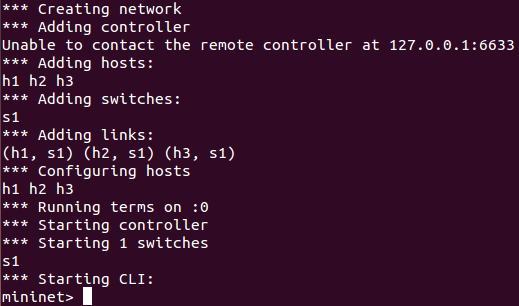
\includegraphics[width=0.40\textwidth]{./pictures/mininet.png}
	\caption{Mininet start}
	\label{x}
	\end{center}
\end{figure} 

\subsection{OpenFlow}
Hier teilen wir der Bridge mit welche OpenFlow Version verwendet werden soll. Dieser Befehl muss auf s1 ausgeführt werden. 
\begin{lstlisting}
ovs-vsctl set Bridge s1 protocols=OpenFlow13
\end{lstlisting}

\subsection{Ryu application starten}
Nachdem die obigen Vorbereitungen getroffen wurden, können wir jetzt Ryu starten mit dem erstelltem Script als Parameter. Dieser Befehl muss auf dem erstelltem Controller c0 ausgeführt werden. Auch dieser Befehl kann je nach Aufgabe variieren. (Beispiel Ryu Start aus Aufgabe 1) 
\begin{lstlisting}
ryu-manager --verbose simple_hub_v2.py
\end{lstlisting}
\begin{figure} [H]
	\begin{center}
	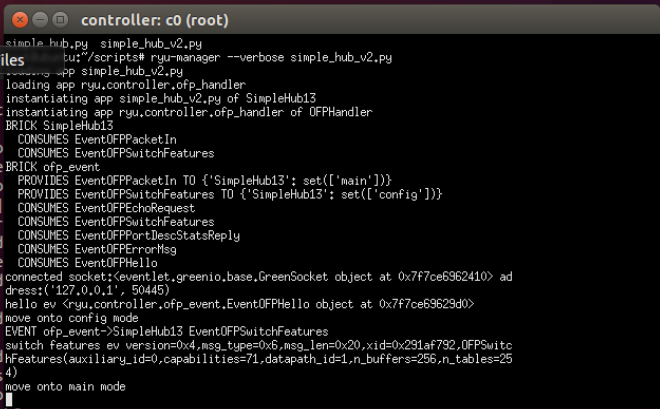
\includegraphics[width=0.50\textwidth]{./pictures/ryu_start_simple_hub.png}
	\caption{Ryu application start}
	\label{x}
	\end{center}
\end{figure} 

\subsection{andere Hilfreiche Befehle}
\subsubsection{Flow Table anzeigen}
Befehl auf s1 ausführen um die Flow Table anzuzeigen. 
\begin{lstlisting}
ovs-ofctl -O OpenFlow13 dump-flows s1
\end{lstlisting}
\newpage

\section{Implementing a Hub - Part 1}

\subsection{Aufgabenstellung}
Wurde aus der Aufgabenstellung entnommen: \\
\\
To get familiar with SDN controller programming you will start with a very basic and easy implementation task. The goal of this exercise is to write a hub.
\begin{itemize}
\item OpenFlow-Switch with Hub behavior
\item Each incoming packet on the OpenFlow-Switch generates a request which will be send to your SDN controller
\item The SDN controller responds to each request with a "FLOOD"-message.
\end{itemize}

\subsection{Ziel der Aufgabe}
Jeder Traffic soll über den Controller gehen, mittels OpenFlow. 

\subsection{Simple Hub Script (Python)}
\begin{lstlisting}
#!/usr/bin/env python
from ryu.base import app_manager
from ryu.controller import ofp_event
from ryu.controller.handler import CONFIG_DISPATCHER, MAIN_DISPATCHER
from ryu.controller.handler import set_ev_cls
from ryu.ofproto import ofproto_v1_3
from ryu.lib.packet import packet

class SimpleHub13(app_manager.RyuApp):
    OFP_VERSIONS = [ofproto_v1_3.OFP_VERSION]

    def __init__(self, *args, **kwargs):
        super(SimpleHub13, self).__init__(*args, **kwargs)

    @set_ev_cls(ofp_event.EventOFPSwitchFeatures, CONFIG_DISPATCHER)
    def switch_features_handler(self, ev):
        datapath = ev.msg.datapath
        ofproto = datapath.ofproto
        parser = datapath.ofproto_parser
        match = parser.OFPMatch()
        actions = [parser.OFPActionOutput(ofproto.OFPP_CONTROLLER, 
        		ofproto.OFPCML_NO_BUFFER)]
        self.add_flow(datapath, 0, match, actions)

    def add_flow(self, datapath, priority, match, actions):
        ofproto = datapath.ofproto
        parser = datapath.ofproto_parser
        inst = [parser.OFPInstructionActions(
        			ofproto.OFPIT_APPLY_ACTIONS, actions)]
        mod = parser.OFPFlowMod(datapath=datapath, priority=priority, 
        				match=match, instructions=inst)
        datapath.send_msg(mod)

    @set_ev_cls(ofp_event.EventOFPPacketIn, MAIN_DISPATCHER)
    def _packet_in_handler(self, ev):
        msg = ev.msg
        datapath = msg.datapath
        ofproto = datapath.ofproto
        parser = datapath.ofproto_parser
        in_port = msg.match['in_port']
        out_port = ofproto.OFPP_FLOOD
        actions = [parser.OFPActionOutput(out_port)]

        data = None
        if msg.buffer_id == ofproto.OFP_NO_BUFFER:
            data = msg.data

        out = parser.OFPPacketOut(datapath=datapath, 
        	buffer_id=msg.buffer_id, in_port=in_port, 
        		actions=actions, data=data)
        datapath.send_msg(out)
        dpid = datapath.id
        self.logger.info("packet in %s %s", dpid, in_port)
\end{lstlisting}
\newpage

\subsection{Traffic}
Nachdem alles gestartet wurde können wir im Mininet von Host (h1) zu Host (h3) pingen um zu sehen ob der Verkehr mittels OpenFlow fliesst. Der Verkehr können wir mit Hilfe von Wireshark sniffen. Der gesamte Traffic verläuft über den Controller c0. Jedes Paket wird in ein OpenFlow Paket gekapselt und weitergeleitet. Der Hub ist nicht in der Lage einen Flow zu lernen. 
\begin{figure} [H]
	\begin{center}
	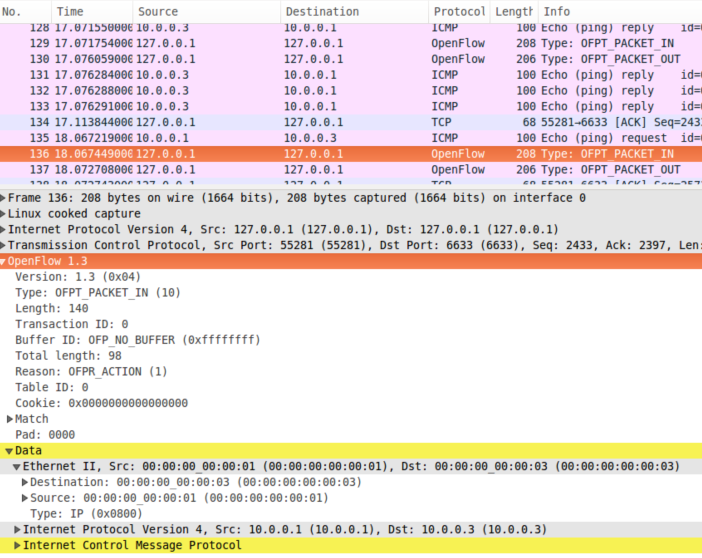
\includegraphics[width=1.00\textwidth]{./pictures/simple_hub_traffic.png}
	\caption{Mininet Traffic ping from h1 to h3}
	\label{x}
	\end{center}
\end{figure} 
\newpage

\section{Implementing a Hub - Part 2}

\subsection{Aufgabenstellung}
Wurde aus der Aufgabenstellung entnommen: \\
\\
In the second part of the hub implementation you will improve the hub behavior as follows:
\begin{itemize}
\item Still Hub behavior
\item During the connection setup between the OpenFlow-Switch and your SDN-Controller the controller installs a flow on the OpenFlow-Switch:  Flow: always Flood
\end{itemize}

\subsection{Ziel der Aufgabe}
Jeder, nicht bekannte Flow, soll an den Controller gesendet werden. 

\subsection{Infrastruktur}
An der Infrastruktur ändert sich für diese Aufgabe nur das Script. Ansonsten dieselbe wie 1.1.3. 

\subsection{Simple Hub Flood Script (Python) }
\begin{lstlisting}
#!/usr/bin/env python
from ryu.base import app_manager
from ryu.controller import ofp_event
from ryu.controller.handler import CONFIG_DISPATCHER, MAIN_DISPATCHER
from ryu.controller.handler import set_ev_cls
from ryu.ofproto import ofproto_v1_3
from ryu.lib.packet import packet

class SimpleHub13(app_manager.RyuApp):
    OFP_VERSIONS = [ofproto_v1_3.OFP_VERSION]

    def __init__(self, *args, **kwargs):
        super(SimpleHub13, self).__init__(*args, **kwargs)

    @set_ev_cls(ofp_event.EventOFPSwitchFeatures, CONFIG_DISPATCHER)
    def switch_features_handler(self, ev):
        datapath = ev.msg.datapath
        ofproto = datapath.ofproto
        parser = datapath.ofproto_parser
        match = parser.OFPMatch()
        actions = [parser.OFPActionOutput(ofproto.OFPP_CONTROLLER, 
        		ofproto.OFPCML_NO_BUFFER)]
        self.add_flow(datapath, 0, match, actions)

    def add_flow(self, datapath, priority, match, actions):
        ofproto = datapath.ofproto
        parser = datapath.ofproto_parser
        inst = [parser.OFPInstructionActions(
        			ofproto.OFPIT_APPLY_ACTIONS, actions)]
        mod = parser.OFPFlowMod(datapath=datapath, priority=priority, 
        				match=match, instructions=inst)
        datapath.send_msg(mod)

    @set_ev_cls(ofp_event.EventOFPPacketIn, MAIN_DISPATCHER)
    def _packet_in_handler(self, ev):
        msg = ev.msg
        datapath = msg.datapath
        ofproto = datapath.ofproto
        parser = datapath.ofproto_parser
        in_port = msg.match['in_port']
        out_port = ofproto.OFPP_FLOOD
        actions = [parser.OFPActionOutput(out_port)]

	match = parser.OFPMatch()
	self.add_flow(datapath, 1, match, actions) 
		
        data = None
        if msg.buffer_id == ofproto.OFP_NO_BUFFER:
            data = msg.data

        out = parser.OFPPacketOut(datapath=datapath, 
        	buffer_id=msg.buffer_id, in_port=in_port, 
        		actions=actions, data=data)
        datapath.send_msg(out)
        dpid = datapath.id
        self.logger.info("packet in %s %s", dpid, in_port)
\end{lstlisting}
\newpage 

\subsection{Traffic}
Durch einen ICMP Test im Mininet ist gut sichtbar wie sich der Flow verhält. Der Erste Pring hat eine deutlich höhere Round Trip Time als die restlichen. Dieser ist höher weil, der Flow zu dieser Zeit noch nicht bekannt ist, die restlichen Pings werden direkt gefloodet und haben deshalb eine geringere Round Trip Time. 
\begin{figure} [H]
	\begin{center}
	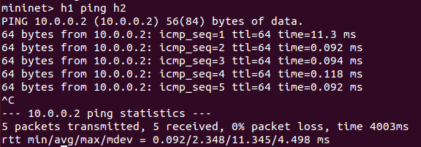
\includegraphics[width=1.00\textwidth]{./pictures/ping_test1_flood.png}
	\caption{Mininet Traffic ping from h1 to h2}
	\label{x}
	\end{center}
\end{figure} 

\subsubsection{Flow Table}
Wenn man die Flow Table anzeigen lässt sind jetzt mehrere Einträge vorhanden. Man erkennt daraus den Pfad mit Priorität 0: Controller, und den Pfad mit Priorität 1: Flood. Eine weitere wichtige Erkennung ist die Anzahl Pakete. Unter dem Eintrag mit Priorität 0 ist zu sehen das sich die Anzahl Pakete auf eines beschränkt, und der Pfad mit Priorität 1 die restlichen Pakete des flows enthält. 
\begin{figure} [H]
	\begin{center}
	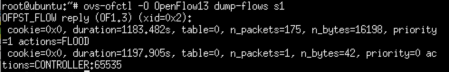
\includegraphics[width=1.00\textwidth]{./pictures/flow_table_flood.png}
	\caption{Mininet Traffic ping from h1 to h2}
	\label{x}
	\end{center}
\end{figure} 
\newpage

\section{Implementing a Switch}

\subsection{Aufgabe}
Wurde aus der Aufgabenstellung entnommen: \\
\\
Now you should be familiar with the functionality of the RYU SDN controller. In this exercise you will write a learning switch. This is more challenging than the hub implementation. The following steps should guide you:
\begin{itemize}
\item OpenFlow-Switch: Packet incoming\\
Existing flow?\\
No flow: send to controller
\item Learn source MAC address and incoming port
\item Write into table
\item  Destination MAC address already in table?\\
Yes, forward packet only to outgoing port: install flow on Switch\\
No, flood packet to all ports, except the incoming port
\item Existing flow
\item Forward as specified
\end{itemize}

\subsection{Ziel der Aufgabe}


\end{document}